%=== Préambule ===========================================================

\documentclass[aspectratio=169]{beamer}
\usepackage[english]{babel}
\usepackage{xspace}
\usepackage{hyperref}
\usepackage{listings}
\usepackage{csquotes}
\usepackage{graphicx}
\usepackage{wrapfig}
\usepackage{pdfpages}
\usepackage{tikz}
\usepackage{natbib}

\uselanguage{English}
\languagepath{English}
\setcounter{tocdepth}{1}

\lstset{
  numbers=left,
  basicstyle=\tiny\ttfamily,      
  breaklines=true, 
  showtabs=false,
  showstringspaces=false,
}  

%=== Configuration de Beamer et du thème metropolis ======================

\usetheme[background=light]{metropolis}

\definecolor{mLightBrown}{HTML}{000000}
\definecolor{black}{HTML}{000000}
\setbeamercolor{structure}{fg=black,bg=mLightBrown}
\setbeamercolor{palette primary}{%
	use=normal text,
	fg=normal text.bg,
	bg=mLightBrown
}
%\setsansfont[BoldFont={Linux Libertine G Bold},Numbers={OldStyle}]{Linux Libertine G}

\metroset{block=fill}

%=== Page de titre =======================================================

%path to logo and biblio -> to be adapted to your local directories 
\newcommand\dirlogo{~/Public/hugosanrocks.github.com/tex_documents/logos/}
\newcommand\dirbiblio{../../biblio/,/}



\title{{\vskip 1.5cm Curso 1: Teor\'ia de inversi\'on y programaci\'on en Python}}
\subtitle{}
\author{H. S\'anchez-Reyes}

\institute[ISTerre, Universit\'e de Grenoble Alpes]
{
ISTerre, Universit\'e de Grenoble Alpes, France\\
\textit{IRD - UGA-ISTerre BQR Project} \vskip 1cm
7-18 de Agosto de 2023\\
Lima, Per\'u
}

\date[2023]{}%2020 AGU Fall Meeting, 8th December}
\subject{}

\titlegraphic{\centering \vspace{-15pt}\includegraphics[height=1.2cm]{\dirlogo/IRD.png} \qquad \quad \includegraphics[height=1.2cm]{\dirlogo/UGA} \qquad \quad \includegraphics[height=1.2cm]{\dirlogo/ISTerre} \par \vskip 3cm \hskip 8cm \includegraphics[height=2cm]{\dirlogo/IGP.jpeg}\\ \hskip 8cm ¡Gracias por la bienvenida!}


\addtobeamertemplate{frametitle}{}{%
\begin{tikzpicture}[remember picture,overlay]
  \node[anchor=north east,yshift=0.0ex] at (current page.north east) {\includegraphics[height=4ex]{\dirlogo/IRD_inv.png}};
  %\node[anchor=north east,yshift=0.5ex] at (current page.north east) {\includegraphics[height=3.3ex]{\dirlogo/seiscope_color_light_background}};
\end{tikzpicture}}



%=== Document ============================================================

\begin{document}

% --- Préambule ---------------------------------------------------------------

\begin{frame}
    \titlepage
\end{frame}

\section{\small Recordando algebra lineal}

\begin{frame}
 {Vectores, matrices, elementos y operaciones b\'asicas}
 
 \vskip -0.1cm
 Vectores: 
 \begin{equation*}
  v = [2, 4, 5] \qquad  \textnormal{or,} \qquad n = 
  \begin{bmatrix}
  1 \\ 5 \\ 7    
  \end{bmatrix}
 \end{equation*}
\pause
 \vskip -0.4cm
¿Cu\'al es la dimensi\'on de estos vectores? \pause
 \vskip -0.4cm
 \begin{equation*}
  v = [2, 4, 5]_{1\times3} \qquad  \textnormal{or,} \qquad n = 
  \begin{bmatrix}
  1 \\ 5 \\ 7    
  \end{bmatrix}_{3\times1}
 \end{equation*}
 \pause
 \vskip -0.4cm
 Tambi\'en definimos los transpuestos:
 \vskip -0.4cm
 \pause
 \begin{equation*}
  v^T =
  \begin{bmatrix}
   2 \\ 4 \\ 5
  \end{bmatrix}_{3\times1} \qquad  \textnormal{or,} \qquad n^T = 
  [1, 5, 7]_{1\times3}
 \end{equation*}

\end{frame}


\begin{frame}
 {Vectores, matrices, elementos y operaciones b\'asicas}

 Matrix:
 \begin{equation*}
  \begin{bmatrix}
   4 & 1 & 0 \\
   2 & 7 & 2 \\
   5 & 3 & 8 
  \end{bmatrix}_{3\times3}
 \end{equation*}
 \pause
Matrices con definiciones importantes
 \begin{equation*}
 \textnormal{Identidad:} \pause \quad I = \begin{bmatrix}
   1 & 0 & 0 \\
   0 & 1 & 0 \\
   0 & 0 & 1 
  \end{bmatrix} \pause \qquad 
   \textnormal{Sim\'etricas:} \pause \quad X = \begin{bmatrix}
   x_{11} & x_{12} & x_{13} \\
   x_{21} & x_{22} & x_{23} \\
   x_{31} & x_{32} & x_{33} 
  \end{bmatrix} \quad \textnormal{si}, x_{ij} = x_{ji} 
 \end{equation*} \pause
 Invertible: \pause \quad si, \quad $\det(M) > 0$ \quad entonces, \quad $M^{-1}$ existe, tal que 
 \begin{equation*}
  M^{-1}M = I = MM^{-1}
 \end{equation*}
 \pause \vskip -1.4cm
 \begin{equation*}
  \underbrace{M^{-1}}_{pre-multiplicar}M = I = M\underbrace{M^{-1}}_{post-multiplicar}
 \end{equation*}

\end{frame}


\begin{frame}
 {Vectores, matrices, elementos y operaciones b\'asicas}

 \vskip 0cm
 Sumas (y restas): 
 \begin{center}  
 \vskip -1cm
 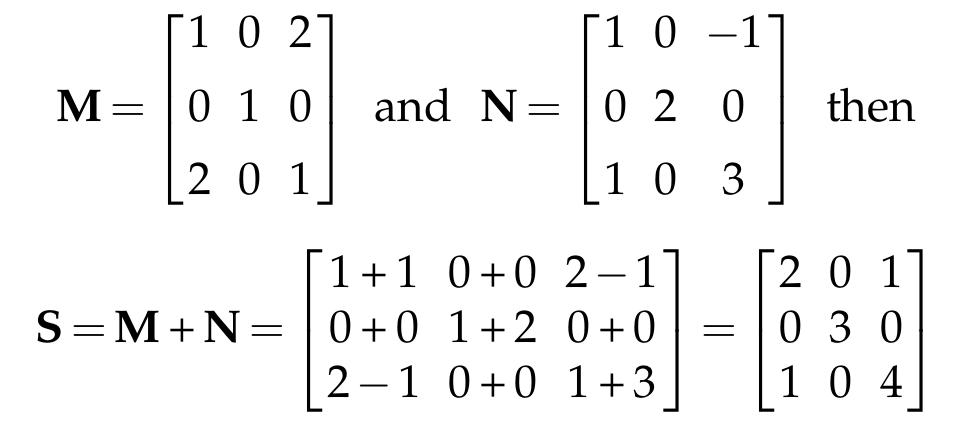
\includegraphics[width=0.5\linewidth]{images/sum_matrix.png} \\ \pause
 es decir, $S_{ij} = M_{ij} + N_{ij}$ \quad y \quad $D_{ij} = M_{ij} - N_{ij}$
 \end{center}
 \pause
\vskip -0.3cm Multiplicaciones: \pause
 \begin{center}
 \vskip -0.4cm 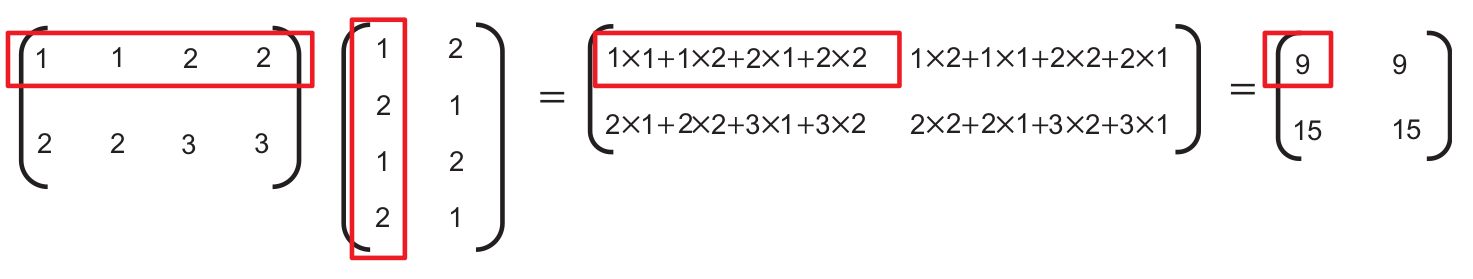
\includegraphics[width=0.9\linewidth]{images/multiplication.png} \\ \pause
 \vskip -1.2cm es decir,
 \vskip -0.8cm \begin{equation*}
  P_{ij} = \sum^{K}_{k=1} M_{ik}N_{kj}
 \end{equation*}
 \end{center}

\end{frame}

\begin{frame}
 {Vectores, matrices, elementos y operaciones b\'asicas}
 
 Determinante: \pause
 \begin{equation*}
  \sum^N_{i=1}  \sum^N_{j=1}  \sum^N_{k=1} \dots \sum^N_{q=1} e^{ijk\dots q} M_{1i} M_{2j} M_{3k} \dots M_{Nq}
 \end{equation*} 
siendo $e^{ijk\dots q} +1$ cuando (i, j, k, ... , q) son permutations pares de (1, 2, 3, ... , N), y $-1$ cuando son permutaciones impares, y cero en otro caso.
 \pause
 \begin{equation*}
  \det{\begin{bmatrix}
        a & b \\
        c & d 
       \end{bmatrix}} = ad - bc
 \end{equation*}

 
\end{frame}

\begin{frame}
 {Vectores, matrices, elementos y operaciones b\'asicas}

 \begin{center}
  \Large M\'as in \cite{Menke_2018_GEO}
 \end{center}
 
\end{frame}

\section{\small I. Problema directo / Forward problem}

\section{\small II. Problema inverso / Inverse problem}

\section{\small III. Problema lineal / Linear problem}

\section{\small IV. Problema no-lineal / Non-linear problem}

\begin{frame}

    \bibliography{biblio}
    \bibliographystyle{apalike}    

\end{frame}


\end{document}

